\chapter[Design af software]{Software}

% Note om hvad der skal stå i dette afsnit her.


\section{Motorstyring}

\mnote{Kristian Kjærgaard}

Dette afsnit diskuterer forskellige metoder til at styre tegnehovedets
placering.

Hastigheden for tegnehovedet er givet ved
\begin{align}
  v = \frac{\Delta x}{\Delta t} \label{eq:hastighed}
\end{align}
hvor $v$ er hastigheden, $\Delta x$ er positionsændring og $\Delta t$ er
tidsændring. En præcis styring af hastighed kræver et præcist kendskab
til både positionsændring og tidsændring.

Den mindst mulige positionsændring er ét step med stepmotoren og
kendskabet til denne er tilstrækkeligt.

Følgende to afsnit diskuterer to forskellige metoder til at
\textit{time} motorerne.


\subsection{Motorstyring med indlagt forsinkelse}

En metode at styre timingen på er ved at afvikle tidsberegningen på en
tråd med indlagt forsinkelse, således at vi beregner den tid $\Delta t
= \frac{\Delta x}{v}$, vi skal vente, se
figur\vref{fig:motorstyring-indlagt-forsinkelse}.

\begin{figure}[htbp]
  \centering
  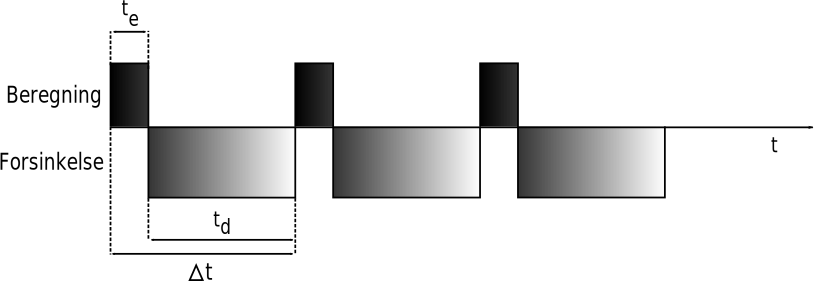
\includegraphics[width=.8\textwidth]{./img/motorstyring-indlagt-forsinkelse}
  \caption{Motorstyring med indlagt forsinkelse.}
  \label{fig:motorstyring-indlagt-forsinkelse}
\end{figure}


For denne metode gælder, at tidsændringen $\Delta t$ er summen af den
tid, det tager af afvikle beregningen $\frac{\Delta x}v$ og den tid,
der indlægges som forsinkelse:
\begin{align}
  \Delta t &= t_e + t_d \Rightarrow \label{eq:afbrudt-afvikling-tid} \\
  v &= \frac{\Delta x}{t_e + t_d}
\end{align}
hvor $t_d$ er den indlagte forsinkelse og $t_e$ er den tid det tager
at afvikle tidsberegningen (se
figur\vref{fig:motorstyring-indlagt-forsinkelse}).

Ekserkveringstiden $t_e$ kan variere og kendes ikke på
afviklingstidspunktet. Derfor er metoden upræcis -- specielt ved høje
hastigheder. Figur\vref{fig:motorstyring-indlagt-forsinkelse-timing}
viser, hvordan $t_e$ får større indflydelse på $\Delta t$ ved høje
hastigheder.

% lav skitse der viser t_e over delta t som funktion af v
\fixme{ny skitse - se kommentar}

\begin{figure}[htbp]
  \centering
  \vspace{3cm}
  \caption{Hastighed som funktion af forsinkelse for motorstyring med
    indlagt forsinkelse.}
  \label{fig:motorstyring-indlagt-forsinkelse-timing}
\end{figure}


\subsection{Motorstyring med afbrudt afvikling}

Alternativt kan motorerne times med afbrudt afvikling. Tiden går mens
det beregnes til hvilket tidspunkter, motorerne skal køres frem til
næste step. Når vi når til et sådant tidspunkt, afbrydes afviklingen
af tidsberegningen mens motorerne flyttes. Når motorerne er flyttet,
genoptages afviklingen af tidsberegningen, se
figur\vref{fig:motorstyring-afbrudt-afvikling}.

\begin{figure}[htbp]
  \centering
  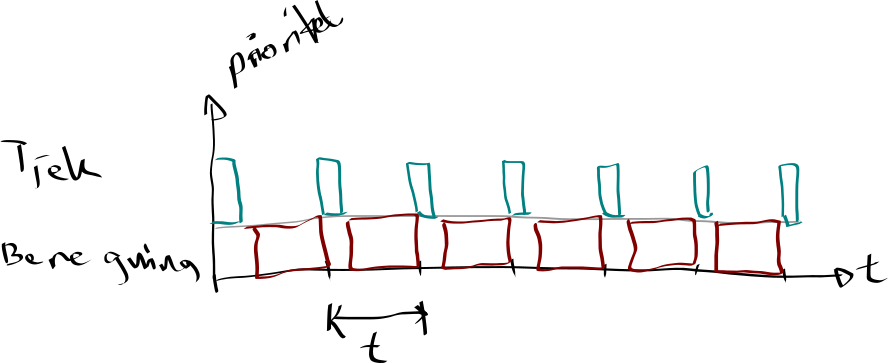
\includegraphics[width=.8\textwidth]{../brugere/kjaergaard/motorstyring-afbrudt-afvikling}
  \caption{Motorstyring med afbrudt afvikling.}
  \label{fig:motorstyring-afbrudt-afvikling}
\end{figure}


Den algoritme, der beregner næste tidspunkt, motorerne skal flyttes
på, afvikles hele tiden. Når det er tid til at tjekke, om vi har
overskredet et tidspunkt, afbrydes afviklingen af tidsberegningen,
mens motorerne flyttes. Bagefter fortsættes afviklingen af
tidsberegningen.

Denne løsning udmærker sig ved at graden af præcis styring af
hastigheden ikke afhænger af hastigheden selv, så længe afviklingen
kan foretages inden en \textit{deadline} nåes.

Løsningen forudsætter, at
\begin{itemize} \firmlist
\item der periodisk tjekkes, om vi har overskredet et tidspunkt,
\item dataene fra algoritmen, der beregner tidspunkter, kan opbevares
  i en kø (først-ind-først-ud struktur, bruges ofte som
  \textit{buffer}),
\item der er data i køen, når det tjekkes, om vi har overskredet et
  tidspunkt, og
\item tidsberegningen kan afvikles så hurtigt, at der lægges data i
  køen hurtigere end der periodisk tjekkes for data.
\end{itemize}


\subsection{Algoritme til tidsberegning}

\mnote{Christian Klim Hansen}

Forholdet imellem tiden det tager at tegne linjen og tiden til et
punkt $x$ linjen lig forholdet imellem det givne punkts $x$-koordinat
og forskellen imellem start- og slutkoordinat $\Delta x$:
\begin{align}
  \frac{t}{\Delta t} &= \frac{x}{\Delta x} \qquad \Rightarrow \nonumber \\
  x &= \Delta x \times \frac{t}{\Delta t} \label{eq:x-af-dxtdt}
\end{align}

Her forudsættes det, at hele linien tegnes med konstant hastighed. Se
figur\vref{fig:matematik-skitse} for geometrisk fremstilling.

\mnote{
  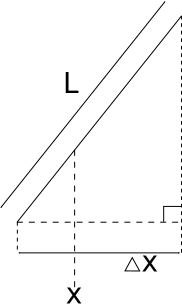
\includegraphics[width=\marginparwidth]{./img/matematik-skitse}
  \captionof{figure}{Tekst her}
  \label{fig:matematik-skitse}
}
\fixme{passende tekst til figur}

Den tid $\Delta t$, det tager at tegne linien, er givet ved
\begin{align}
\Delta t = \frac Lv \label{eq:v-af-lv}
\end{align}

Vi kombinerer \eqref{eq:x-af-dxtdt} og \eqref{eq:v-af-lv} og isolerer
$t$:
\begin{align}
t \times \frac{\Delta x}x &= \frac Lv \Leftrightarrow \\
t &= \frac{\Delta x}x \times \frac Lv \label{eq:t-af-dxxlv}
\end{align}

Længden af linjen $L$ er givet ved
\begin{align}
L &= \sqrt{\left(\Delta x\right)^2 + \left(\Delta y\right)^2}
\end{align}

Forholdet imellem position $x$ og positionsændring $\Delta x$ er lig
forholdet mellem step $n_x$ og stepændring $\Delta n_x$:
\begin{align}
\frac{x}{\Delta x} = \frac{n_x}{\Delta n_x} \label{eq:xdx-af-nxdnx}
\end{align}

Sætning \eqref{eq:t-af-dxxlv} og \eqref{eq:xdx-af-nxdnx} kombineres
til udtrykket
\begin{align}
t &= \frac{n_x}{\Delta n_x} \times \frac{L}{v}
\end{align}

Opløsningen for $x$-retningen er givet ved
\begin{align}
  n_x = x \times \eta_x
\end{align}

Alle symboler med indeks $x$ gælder kun for $x$-aksen. Der arbejdes
med tilsvarende symboler med indeks $y$ for $y$-aksen.


\section{HPGL -- Hewlett-Packard Graphics Language}
\label{sec:hpgl}

Når man skal vælge, hvilket format man vil bruge, når man laver en
plotter, så er der en del ting at tage hensyn til. Der findes mange
forskellige standarder, som kan anvendes og en af disse standarder er
HPGL, som vi benytter os af. Når man skal vælge, hvad man vil bruge, så er det vigtigt at se på
fordele og ulemper.

\begin{table}[htbp]
  \centering
  \caption{Fordele og ulemper ved eget dataformat}
  \begin{tabular}{p{5cm} p{5cm}}
    \toprule
    % vil gerne have \centering på de to overskrifter men kan ikke
    % finde ud af det
    \bfseries Fordele & \bfseries Ulemper \\
    \midrule
    { \begin{itemize} \firmlist
      \item Vi kan gøre det så simpelt som muligt, både til at læse og
        til at forstå
      \end{itemize} }
    &
    { \begin{itemize} \firmlist
      \item Det vil nok afføde børnesygdomme
      \item Der findes ikke software, som kan håndtere vores
        dataformat
      \end{itemize} } \\
    \bottomrule
  \end{tabular}
\end{table}
\fixme{Fix layout på tabel (punktform?)}

Vi kunne i princippet godt udvikle vores eget
plotterformat, men dette vil både være meget tidskrævende, og
samtidigt vil det være svært at få implementeret, da vores format ikke
er en standard, og derfor er der ikke noget som direkte virker med
det. Derfor er HPGL velegnet i vores projekt, da det er mere
virkelighedsnært at benytte en standard, som allerede er konstrueret
som et plotterformat, samtidig med at det kan anvendes af forskellige
applikationer (andre CAD programmer). Der er heller ikke mange ulemper
tilknyttet til brugen af HPGL som plotterformat. Det vil dog tage lang
tid at implementere det hele, hvilket vi dog heller ikke gør. Vi
kommer f.eks. ikke til at benytte os af pin-skrift og en del andre
ting, men disse problemer er relativt lette at komme udenom. Figur
\vref{tab:hpgl-fordele-ulemper} viser vores overvejelser om brugen
af HPGL som dataformat.

%Når man betragter HPGL som et plotterformat, så betyder det, at den
%indeholder mange forskellige kommandoer med hver deres funktion. Det
%kan tage lang tid at sætte sig ind i alle disse ting, men hvis man har
%forståelse for, hvilke funktioner vi evt. kommer til at bruge i vores
%projekt, vil det selvfølgelig lette indlæringsarbejdet en del.

%Følgende er en tabel over vores overvejelser omkring fordele og
%ulemper ved brugen af eget dataformat samt fordele og ulemper ved
%brugen af HPGL:

%Dette betyder, at der findes ingen software, der kan håndtere
%formatet. Dette betyder at vi selv skal skrive den software, som er
%uden for rammer af dette projekt. Derfor leder vi efter en
%eksisterende standard.


\begin{table}[htbp]
  \centering
  \caption{Fordele og ulemper ved HPGL.}
  \label{tab:hpgl-fordele-ulemper}

  \begin{tabular}{p{5cm} p{5cm}}
    \toprule
    Fordele & Ulemper \\
    \midrule
    { \begin{itemize} \firmlist
      \item Afprøvet og bruges industrielt til plottere
  	  \item Veldokumenteret
      \item Der findes software, som kan håndtere HPGL
      \end{itemize} }
    &
    { \begin{itemize} \firmlist
      \item Niveauet er sat højt, hvilket betyder, at der er mange
        funktioner som vi ikke får brug for
      \item Implementeringstiden er længere
      \end{itemize} }
    \\
    \bottomrule
  \end{tabular}
\end{table}

Dette betyder, at HPGL er meget velegnet til brug i vores projekt, da
formatet er veldokumenteret, afprøvet og anvendt industrielt til
specielt plottere, hvilket vores eget selvfølgelig også ville være, og
der finde allerede software, som kan håndtere formatet til forskel fra
vores eget. Implementeringstiden vil dog være en del længere, da
niveauet er sat fra starten, hvilket medfører en del ubenyttede
funktioner.


\section{Koordinatsystem}
\mnote{Kristian Kjærgaard}

% Skriv om koordinatsystemet

Vi arbejder med skærmkoordinater (se
figur\vref{fig:skaermkoord}). HPGL (se afsnit\vref{sec:hpgl}) er
formateret i skærmkoordinater (Cartesiansk koordinatsystem med én
kvadrant, $x$-akse voksende mod højre og $y$-akse
voksende ned), og internt i softwaren kan en konvertering springes
over ved at bruge skærmkoordinater.

\mnote{
  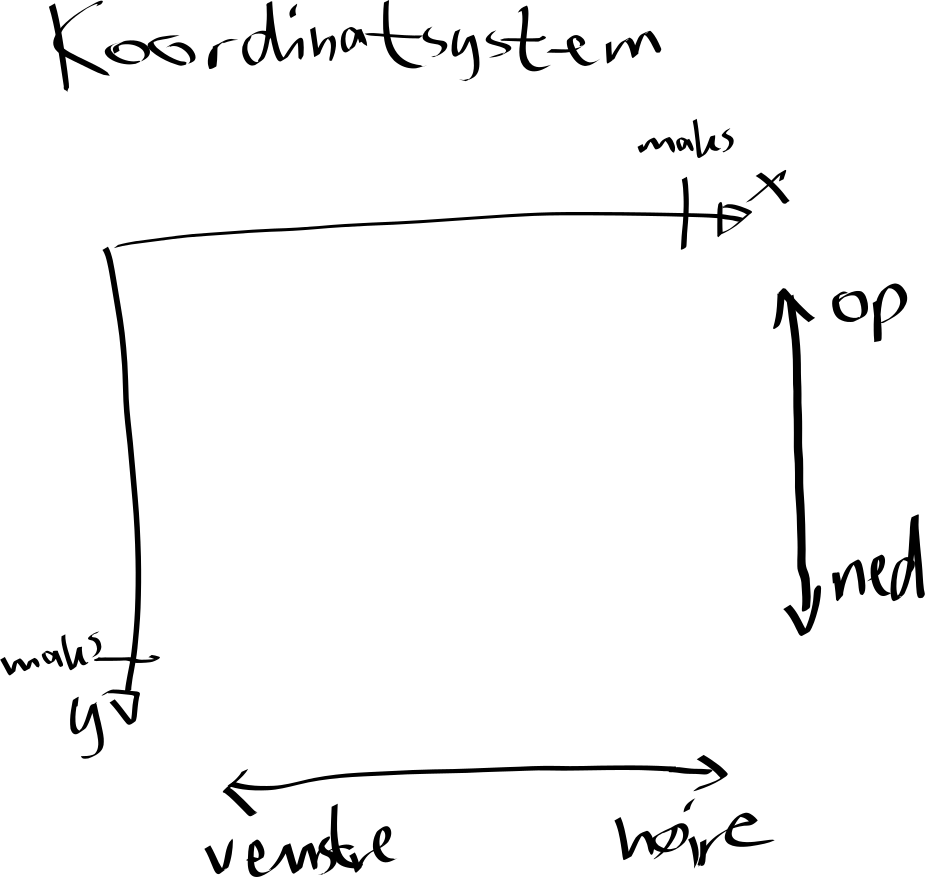
\includegraphics[width=\marginparwidth]{../brugere/kjaergaard/skaermkoordinater}
  \captionof{figure}{Skærm\-koor\-dinater. Der arbejdes med
    skærm\-koordinater i plotteren.}
  \label{fig:skaermkoord}
}

\section[Valg af programmeringssprog]{Valg af
  programmeringssprog\footnote{Se rettelser til dette afsnit i afsnit\vref{sec:bilag-programmeringssprog}}}
\fixme{henvisning}

Softwaren skrives i C og \Cpp.

C bruges i moduler, hvor sproget uden videre er tilstrækkeligt. Dette
vil typisk være lavniveaumoduler, og her er C fordelagtigt, fordi det
giver større kontrol.

\Cpp\ bruges i moduler, hvor det er fordelagtigt at bruge
\Cpp-speficikke elementer (f.eks. generisk programmering\fixme{note om
  dette?}). Moduler, der afhænger af moduler skrevet i \Cpp, vil
typisk også være skrevet i \Cpp.

Alle C-moduler er kompatible med \Cpp, og alle \Cpp-moduler er så vidt
muligt kompatible med C. Uønskede sideeffekter af \Cpp\ forsøges
undgået (\fixme{eksempler her!}). \Cpp\ bruges ikke objektorienteret.



%%% Local Variables: 
%%% mode: latex
%%% TeX-master: "../master"
%%% End: